% psrdatamanagement_srs.tex - SRS for the Pulsar Data Management project.

\documentclass[a4paper,11pt]{article}
\usepackage[pdftex]{graphicx}

\headheight 0in
\headsep 0in
\oddsidemargin 0in
\evensidemargin 0in
\textheight 9.5in
\textwidth 6in

\begin{document}

\title{Software Requirements Specification for ATNF Pulsar Data Management}
\author{Jonathan Khoo}
\date{\today}
\maketitle
\clearpage

\section{Introduction}

%\subsection{People Involved}
%Dick Manchester, Matthew Bailes, George Hobbs, Simon Johnston, Mike Keith, Ryan Shannon, Willem van Straten, Andrew Jameson, Phil Edwards, Vince McIntyre, Jessica Chapman, Gina Spratt, Jonathan Khoo

\subsection{Purpose}
This system will be created, with the aim to lower the amount of manual work required and to make the current data transfer more robust. It will automatically transfer certain types of pulsar data \footnote{All fold-mode data from DFBs, APSR, CASPSR, all search-mode data from DFBs less than 2 GB, and AFB data. This excludes BPSR and search-mode data from the DFBs greater than 2GB.}, taken at Parkes, to Epping, and stakeholders will be able to monitor this system via a set of web pages. Software will be developed to perform automated book-keeping at Parkes and Epping.

\subsection{Intended Audience}
As this document details the general features and requirements of the project, it is intended for viewing by all involved (pulsar observers, users at Parkes and Epping, developers, computing staff at Parkes and Epping, and ... ).

\subsection{Document and Project Conventions}
\begin{itemize}
\item \emph{DFBs} refers to both PDFB3 and PDFB4. As these backends are basically identical (regarding this project), for the purpose of documentation in this project, they have been commonly grouped together.
\item \emph{System} is the compilation of all software developed and changes made in this project.
\item \emph{Project} is the overall process of developing the system.
\end{itemize}

\subsection{Project Scope}
Software will be developed in order to perform the automated data transfer from Parkes to Epping from the following backends:
\begin{enumerate}
\item DFB3
\item DFB4
\item AFB
\item APSR
\item CASPSR
\end{enumerate}

Note that BPSR will not be included in this system. However, due to the extensible design of this system, it can be added easily in the future (assuming the necessary disk space at Parkes and Epping is available, and the file format can be converted into the required psrfits format). The development of this system will occur parallel to the current work operations---all observing, and usual data transfer will be unhampered and will continue until the completion of this project. The directory structure at Epping will undergo a large change (see: blahhhhhhhhhhh). Re-structuring of the data disks at Epping will also be done in order to provide a more robust system for the user.

\subsection{References}
\begin{itemize}
\item Project management system: https://pm.atnf.csiro.au/science/projects/psrdatamanagement
\item SVN repository: https://svn.atnf.csiro.au/psrdatamanagement
\end{itemize}

\section{Overall Descriptions}
\subsection{System Perspective}
The current method for transferring data from Parkes to Epping is inpractical and incomplete. It is run manually and relies on multiple people. Presently, there is no way of knowing the current status of the data transfer, what files are where, and what DFB fold-mode data are transferred---no search-mode DFB, APSR, CASPSR, BPSR, or AFB data. A separate project, the ANDS-ATNF data archive, aims to make all Parkes data `discoverable' and searchable. With the current data-transfer system in place, preparing the data for the ANDS-ATNF project requirements is another layer of unnecessarily manual work.

The Pulsar Data Management project will create a system to manage all pulsar data (fold mode and search mode) taken at Parkes. The system, running in the background, will automatically transfer completeted observations from the DFBs (both fold- and search-mode data), AFB (search-mode data), APSR (fold-mode data), and CASPSR (fold-mode data), to Epping. All pulsar data transferred from Parkes to Epping will be in psrfits format with the necessary fields correctly populated (see: a later on blah blah blah). The project will produce a system that will display file and disk-space information, and send notifications whenever needed (ee: more blah blah). The system will be designed in an extensible manner, so the addition of other backends can be easily done.

\subsection{System Features}
\begin{enumerate}
\item Software to transfer pulsar data from Parkes to Epping automatically.
\item A suite of web pages to control and monitor the system.
\item Software to perform various bookkeeping tasks at Epping to pre-process and categorise the pulsar data.
\end{enumerate}

\subsection{Users}
Primarily, the expected users of the control and monitoring web pages are ones that have a vested interest (and responsibility) in the status of the pulsar data disks at Parkes and at Epping. Since the project will restructure disks at Parkes and Epping, the wider pulsar community will be indirectly affected. However, the changes made to the disks at Parkes and Epping will be transparent to the everyday pulsar astronomer.

\subsection{Operating Environment}
The project will be implemented in python, shell scripts, mysql, and PHP. All code will be clearly documented and will reside in the ATNF SVN repository (see 1.5 References). The project management system, Redmine, will be utlised to control and oversee the development process (see 1.5 References).

\subsection{Design and Implementation Constraints}
Required fields in PSRFITS!!!!!!!!!!!!!!!!!!!!!!!!!!!!!!!!!!!

\subsection{User Documentation}
Documentation detailing what has been done will provided upon completion of the project. It will include:
\begin{enumerate}
\item An overview of the data-transfer pipeline.
\item How to use the monitoring web pages.
\item How to add backends to the system.
\end{enumerate}

Additionally, the code documentation and project management system will provide sufficient information for anyone performing maintenance tasks or modification to the system.

\subsection{Assumptions and Dependencies}
The data transfer will assume a uniform directory structure on each computer hosting data, produced from each backend, at Parkes. All data to be transferred to Epping will be in psrfits format.

\subsubsection{DFBs}
Since the data are already in the psrfits format, no further conversion is required. However, re-structuring of directories may be required to implement the chosen backend directory structure.

\subsubsection{AFB}
AFB data will be converted to psrfits (search-mode) format. George Hobbs has code to perform this conversion.

\subsubsection{APSR}
APSR data will be pre-processed and stored on a new RAID from Swinburne that will be available at Parkes around mid-February, 2011. The output will be files in psrfits format, ready to be transferred to Epping and categorised immediately (without further processing). Andrew Jameson is the point of contact for the RAID. I will work with him to gain access to the RAID and deploy the necessary tools to manage APSR data at Parkes.

\subsubsection{CASPSR}
CASPSR data will be processed and available similarly to APSR.

\section{System Features}

\subsection{Web Pages}
The primary interface for the data-transfer pipeline will be online in the form of a suite of web pages. These web pages will be used to control and monitor the system.

\subsubsection{Control}
Control web pages will be accessible after user authentication (only a select number of people will have authorised access). They will provide the functionality to display values from the configuration file such as how often to check for completed observations, time threshold to determine if an observation is complete, etc.
%They will provide the following functionality:

%\begin{enumerate}
%\item Display values from the configuration file (e.g., how often to check for completed observations, time threshold to determine if an observation is complete, etc.).
%\end{enumerate}

\subsubsection{Monitor}
Monitoring web pages will be accessible from any computer within the internal ATNF network. These pages will provide the following functionality:

\begin{enumerate}
\item Completed Parkes observations that are currently in queue, waiting to be copied from Parkes to Epping.
\item Recent successfully copied observations at Epping (time-sorted by default, and grouped by day).
\item Disk-space status for disks at Parkes (DFBs and the RAID containing the APSR and CASPSR data.
\item Disk-space status for disks containing raw pulsar data at Epping.
\item Files at Parkes that have not been backed up.
\item Files at Epping that require attention (e.g., no project ID entered, junk data---only the header information has been written, symlinks that do not point to the raw file correctly etc.).
\item Files at Epping that do not have corresponding existing symlinks in the ANDS-ATNF folder. (Currently, files are collated from one folder which further categorised by project ID.)
\item Search-mode data at Parkes for files greater than 2GB.
\end{enumerate}

\subsection{Data Transfer}

The data transfer can be simplified to:
\begin{verbatim}
for all completed observations: 
  if file (at Parkes) has not been successfully copied to Epping:
    push it into the copy-to-Epping queue

---------------------------------------------------------------

while there are files in the copy-to-Epping queue:
  copy file to Epping
  if checksum is correct (at Epping):
    remove file from copy-to-Epping queue
\end{verbatim}

\subsection{Data Shuffling at Parkes}
Currently, DFB data files are deleted from the Parkes disks as follows:
\begin{itemize}
\item Fold-mode data: when backed up on tape at Parkes and copied to Epping.
\item Search-mode data: when backed up on tape at Parkes.
\end{itemize}

To perform the data removal at Parkes, Dick follows a set of instructions which verifies the data and manually removes the target files. Gina Spratt maintains an email notification which is triggered when a data disk at Parkes is more than 86\% full. John Sarkissian does the tape backup at Parkes. This process should be examined and automated where possible to reduce the overall dependence on multiple people. This system will implement the necessary process to delete files for all backends at Parkes that have been backed up onto tape at Parkes and successfully copied from Parkes to Epping. Extensive testing will be performed before data are deleted automatically. Only psrfits files will be removed in this system. (Other formats produced by APSR, CASPSR, and AFB will be untouched.)

\subsection{Automatic Ingest for ANDS-ATNF}
Conforming with the requirements of the ANDS-ATNF data-archiving project, symlinks to all newly transferred data (and all existing data) will be created and placed in a separate directory tree for ANDS-ATNF. When the data gets copied to Epping, the following pre-processing steps will be performed automatically:

\begin{itemize}
\item Create a fully scrunched (polarisation-, frequency-, and time-scrunched) archive.
\item Create an image of the fully scrunched profile.
\end{itemize}

Symlinks will also be created in the ANDS-ATNF directory tree. The structure of this directory tree is:

\begin{verbatim}
root directory -> project ID -> source name -> data files
\end{verbatim}

Where \emph{root directory} is /pulsar/archive21/ANDS; \emph{project ID} is the value of PROJ\_ID (from the main header of the psrfits file); and, \emph{source name} is either the pulsar name, or the pulsar name with `\_R' appended to it (signifying a calibration file).

\subsection{Directory Structure at Epping}
A new directory structure for the pulsar data at Epping will be defined, implemented, and utlised.

\subsubsection{Folded Data}
Currently, all DFB data (located at Epping) are stored across five `root' directories (i.e., \$DFB1--\$DFB5). The structure is as follows:

\begin{verbatim}
root directory -> source name -> data files
\end{verbatim}

Where \emph{root directory} is \$DFB1--\$DFB5, and \emph{source name} is either the pulsar name, or the pulsar name with `\_R' appended to it (signifying a calibration file). The folders which contain CPSR2 and APSR data have the same structure but are stored, once again, on separate disks. In order to search for data, all five \$DFB directories must be searched. The new directory structure will be something like:

\begin{verbatim}
root directory -> year of observation -> source name -> symlinks to data files
\end{verbatim}

A single folder listing for all data (from all backends) once in the \emph{source name} level. The reason for the additional \emph{year of observation} step is to prevent too many files/symlinks from being contained in a single directory. Mike suggested that the symlink targets can be maintained by using a database which contains the location of the raw data files.

\subsubsection{Search Data}
Currently, search-mode data must be transferred from Parkes to Epping manually. This system will automatically copy all search-mode data less than 2GB and store them in the following directory structure:

\begin{verbatim}
root directory -> year of observation -> identifier -> symlinks to data files
\end{verbatim}

Where \emph{identifier} is either the value of the SRC\_NAME field from the header (that also exists in psrcat), or a folder name containing files from a three-month block. Files greater than 2GB will not be transferred automatically---it will be left to the observer's discretion.

\subsection{Backups}
\subsubsection{Parkes}
Currently, all DFB fold-mode data are backed up onto tape. Search-mode data are deleted when the purges are performed. This will remain the same.

\subsubsection{Epping}
Currently, all DFB fold-mode data are backed up onto tape. This is conducted manually every 1--6 months. The commencement of this project will see both fold- and search-mode data transferred from Parkes to Epping backed up on tape.

\subsection{Other Data-processing Pipelines (PPTA, Fermi, etc.)}
This system will not automatically start other data-processing pipelines (PPTA, Fermi, etc.)---it will be up to the processing pipelines to determine what to do with the data. However, the same database utilised in this system may be queried and cross-checked to create a list of target files that require processing.

\subsection{Project Timeline}
This is a mixture of high- and lower-level tasks required for the completion of this project.

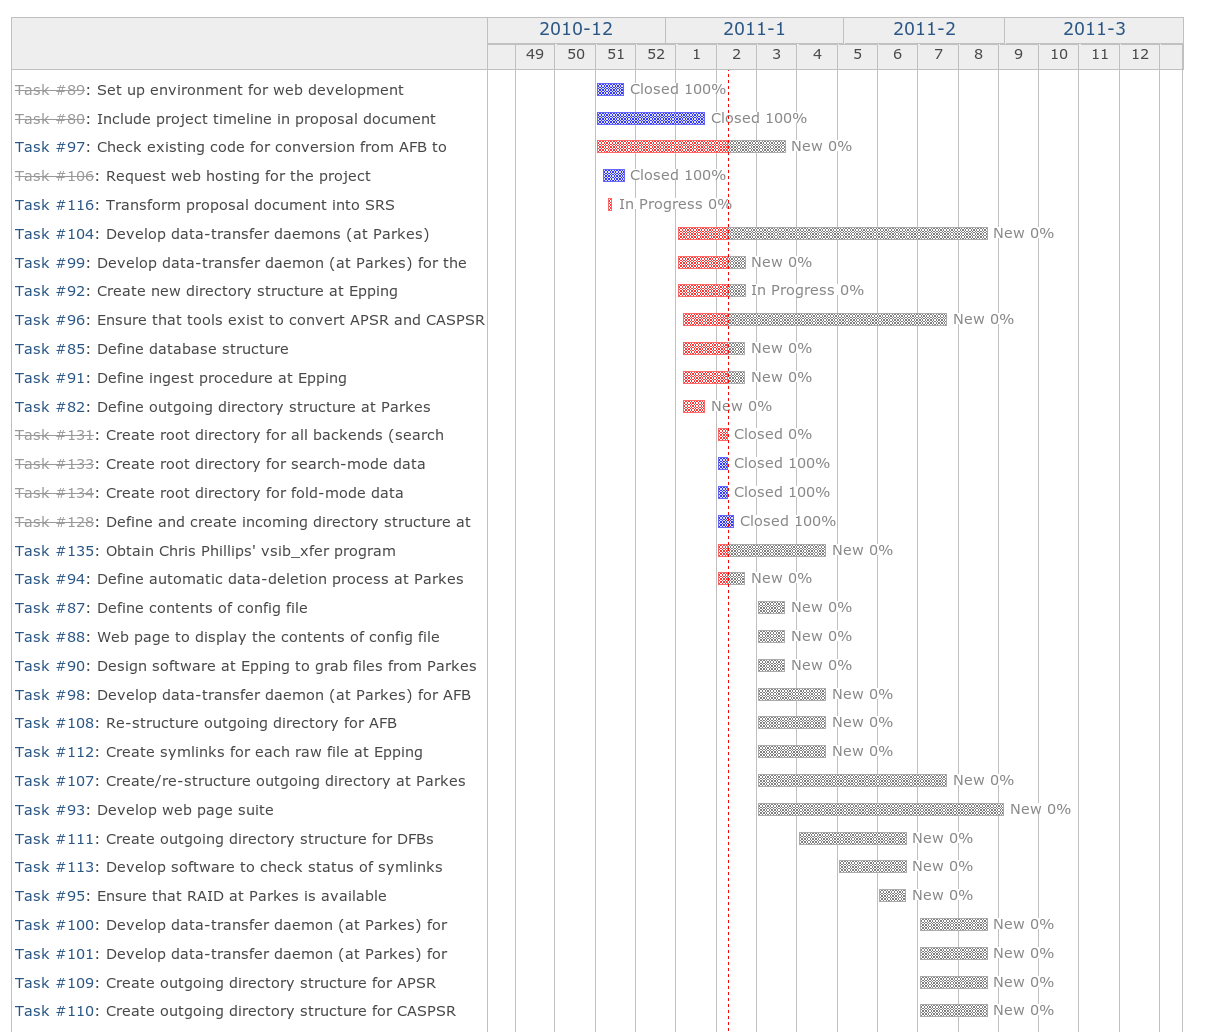
\includegraphics[scale=0.4]{timeline.png}

\end{document}
